%Andy Sayler
%SmartWall Project
%Created April 29, 2011

\documentclass[12pt]{article}
\usepackage[text={6.5in, 9in}, centering]{geometry}
\usepackage{graphicx}
\usepackage{listings}
\lstloadlanguages{C}
\usepackage{amsmath}
\usepackage{url}
\usepackage{pdfpages}

%\usepackage{tikz}
%\usepackage{verbatim}

\lstset{
  language=C,
  basicstyle=\footnotesize,
  numbers=left,
  numberstyle=\footnotesize,
  stepnumber=1,
  numbersep=5pt,
  showspaces=false,
  showstringspaces=false,
  showtabs=false,
  tabsize=4,
  captionpos=b,
  breaklines=false,
  breakatwhitespace=false,
  title=\lstname,
  frame=single,
  frameround=tttt,
  framexrightmargin=3pt,
}

\title{SmartWall: SmartOutlet}
\author{Andy Sayler, Laura Costello, Patrick McKelvy}
\date{\today}

\begin{document}

\maketitle
    
\begin{abstract}

Our team set out to design a system to enable the energy monitoring and
automated control of a collection of in-wall electrical devices and plug-in
appliances. To achieve this goal, we designed the SmartWall protocol,
a self-configuring application layer network protocol for querying and
controlling electrical devices. To demonstrate the power of this protocol
to enable communication and control of in-wall electrical devices, we
designed and prototyped a SmartOutlet. The SmartOutlet is an
intelligent drop-in
replacement for the standard electrical wall outlet that adds the
ability to remotely toggle the outlet plugs on and off and to monitor the
energy usage of any device utilizing the outlet. Finally, we designed a
web based user interface for controlling, administering, and
monitoring our SmartWall network (and any SmartOutlets on it). We hope
this project demonstrates the benefits that come from embedding
standardized energy monitoring and remote control capabilities in
endpoint electrical grid hardware and devices and giving the end user
the ability to control and monitor these devices.
  
\end{abstract}

\pagebreak

\tableofcontents

\pagebreak

\section{Introduction}

\subsection{The Current State}
Currently, residential and business electricity users lack a simple
and affordable means to monitor their energy usage on a per device
level and automate or remotely control electrical devices and
hardware. Even in the 21st century world where most facets of our
lives are accessible from the web and where we can instantaneously
communicate across the globe, we have failed to extend this
connectivity and remote functionality to the basic appliances, devices,
and electrical hardware we use every day. We can process stock trading
orders from our cell phones, or track airline flights from our
laptops, but we can not use these same devices or technologies to turn
the lights out while we're at work or tell us how much energy a
particular appliance is consuming.

\subsection{The SmartWall Vision}
We aim to remedy this technological deficit
by developing a system capable of providing
power monitoring, automation, and remote control
to the end user of any device, appliance, or electrical fixture that
connects to the local electrical system. We call this system
``SmartWall'', reflecting a combination of the current trend
toward assigning an intelligence qualifier to modern ubiquitously
interconnected technologies (\emph{smart}) and the fact that
current electrical systems
revolve around the in-\emph{wall} electrical wiring present in most homes and
office buildings.

The goals of a SmartWall system are as follow:
\begin{description}
  \setlength{\itemsep}{0pt}
  \setlength{\parskip}{0pt}
  \setlength{\parsep}{0pt}
\item[Convenience:] Providing end users with the ability automate and
  control electrically connected devices in their homes from their
  computer, cell phone, or similar device is a desirable convenience
  and one that is currently lacking. From automatically turning lights
  on and off to primitively preheating the oven or turning up the heat
  from work before you arrive home, the SmartWall system adds
  considerable convince and functionality to our day-to-day
  interaction with the devices and appliances we use.
\item[Energy Conservation:] By providing users with the ability to
  monitor their energy usage on a fine grain level and by providing them
  with the ability to programmaticly control the behavior of their electrical
  devices, users have all the necessary tools required for analyzing
  and reducing energy waste. This includes everything from
  automatically turning off unnecessary devices when we are work
  during the day to identifying the largest sources of energy use and
  addressing these sources individually.
\item[Integration Framework:] The SmartWall system lays the groundwork for an
  endless number of integration opportunities with other
  technologies. By providing programmatic and network accessible
  control of the electrical devices and appliances in our homes or
  offices, we open the door for providing a considerable service to any
  number of external systems. From integration with Smart-Grid meters
  that require the ability to turn large appliances on or off at the
  power company's discretion to providing landlords and building
  managers the ability to track energy usage on a per person level and
  bill their tenets accordingly, the possibilities for external
  integration are immense.
\end{description}

The SmartWall vision has three facets:
\begin{description}
  \setlength{\itemsep}{0pt}
  \setlength{\parskip}{0pt}
  \setlength{\parsep}{0pt}
\item[SmartWall Protocol:] The underlying network protocol that
  facilitates communication with and control of SmartWall devices.
\item[SmartWall Enabled Devices:] Any device or electrical fixture that
  connects to the local electrical system and is capable of
  communicating via the SmartWall protocol.
\item[SmartWall User Interfaces:] Any device or system that connects
  the end user to their local SmartWall network for the purpose of
  monitoring, controlling, and/or automating devices on the network.
\end{description}

\subsection{Our Approach}
In line with these three facets, we will be  developing our solution
from three distinct directions:
\begin{description}
  \setlength{\itemsep}{0pt}
  \setlength{\parskip}{0pt}
  \setlength{\parsep}{0pt}
\item[Network:] The SmartWall Network Protocol and Standard
\item[Hardware:] A Proof-of-Concept SmartWall Device - The SmartOutlet
\item[User Interface:] A Proof-of-Concept Web Based User Interface 
\end{description}

Network protocol development involves designing and implementing the
SmartWall protocol governing the communications and command set supported
by our SmartOutlet and our wider SmartWall system suite
vision. We aim for the SmartWall protocol to be open and
extensible. It will fit into the standard IP network stack as an application
layer protocol utilizing the UDP transport layer protocol on top of a
wired, wireless, or power-line Ethernet implementation.

Hardware prototype development encompasses designing,
building, and testing an actual SmartOutlet prototype. The SmartOutlet
aims to be a drop-in replacement for standard in-wall electrical
devices with the added benefits of providing the ability to switch
each socket on or off and
to monitor the power and energy usage of each socket via the SmartWall
network. The hardware prototype will also explore the logistics of
making SmartWall technology affordable: a key prerequisite to ubiquitous
adoption.

User interface development encompasses creating a web based user
interface, as well as any intermediate software that will be necessary
to allow our interface to communicate with our prototype
SmartOutlet(s) via the SmartWall network. This interface will provide
the end user with a simple way to monitor and control their power
consumption on a per device level. It will also allow users the
convenience of automating and remotely controlling devices in their home.

These three sections encompass the necessary tasks that we completed
in reaching our project goal and also reflect the division of labor
between the members of our team. We will reference these three
approaches in the sections below.

\section{Background}

\subsection{Existing Technology}

While the SmartWall system aims to provide energy monitoring and
control capabilities to a wide range of electrical devices, it is not the
first system to offer these services. Several preexisting technologies
of various levels of success already exist in this arena.

The promise of home automation has existed since digital communications
begin to gain prominence in the 1970s. The most extensive effort in this
field is the X10 power-line based automated control system
\cite{wiki-X10}. The X10 system, however, has a number of detractors
that have prevented it from becoming universally deployed:
\begin{itemize}
  \setlength{\itemsep}{0pt}
  \setlength{\parskip}{0pt}
  \setlength{\parsep}{0pt}
\item It is not easily extensible, making it very difficult to add
  support for new devices or for functions beyond simple on/off, dim,
  etc controls.
\item It uses outdated and error-prone power-line communication
  standards making it unsuitable for sending commands over any network
  other than the local power system and causing frequent errors.
\item It does not support power monitoring or more advanced state querying.
\end{itemize}  

There are also a number of products on the market that allow the user
to monitor the energy usage of their devices. P3 Internationale's
``Kill A Watt'' product is a good example of one such a device
\cite{p3-KillAWatt}. Like the X10 system, however, such devices have
failed to gain prominence due to a number of factors including:
\begin{itemize}
  \setlength{\itemsep}{0pt}
  \setlength{\parskip}{0pt}
  \setlength{\parsep}{0pt}
\item They are external, 3rd party devices requiring the consumer to
  purchase an additional power monitor for each electrical device they
  wish to monitor. 
\item They generally provide no networking or remote monitoring capabilities.
\item They are passive monitors, proving no control over devices.
\end{itemize}  

Our SmartWall system combines the benefits of existing automation and
monitoring technologies while addressing their shortcomings and
approaching both capabilities from a 21st century, network-centric approach.

\subsection{Networking}
Ethernet based IP networks have cemented themselves as the standard
for modern communication systems. The IP network stack provides an
abstract, layered approach to network communication. Each layer of the
stack implements specific functionality by relying on the layers below
it and by providing a service to the layers above it. Thus, we can
separate the physical layer, link layer, Internet layer, transport
layer, and application layer and focus on each independently.

The IEEE 1901 ``Homeplug'' collection of power-line Ethernet protocols are
quickly becoming the standard for power-line communications and provide
us with an abstracted power-line communication physical layer on which our
SmartWall system can ride.

The Ethernet link layer provides basic endpoint addressing, error
detection, and packet switching capabilities. As stated above, it is
extremely common technology with a lot of available hardware and
software support.

The IP Internet layer provides global addressing and the ability to
route packets between separate networks. It is the standard Internet layer
for most Ethernet communication and is most frequently used in
conjunction with the TCP or UDP transportation layers.

The UDP transportation layer provides lightweight uni-cast, multi-cast, and
broadcast datagram communication. It has a simple and easy to
implement interface and, along with TCP, is one of the two most common
transportation layers available in the IP stack.

UDP supports an arbitrary application layer protocol. We have
developed the SmartWall protocol to facilitate application layer
communication for this project.

\subsection{Hardware}
The lack of penetration of the existing power monitoring
and automation technologies shows that consumers are unwilling to
spend significantly more money for these capabilities.
Current in-wall electrical fixtures are relatively cheap. A basic outlet
costs only about \$2 and light switches or fixtures are equally
inexpensive. Thus, any technology that aims to become universally
embedded in or bundled with electrical wall-fixtures, devices, and
appliances must not add a considerable cost to these devices.

Monitoring the energy usage of an electrical load involves measuring
the voltage across that load and the current running through it. The
product of those measurements is power: $P = V*I$.  Measuring power is a
simple task for a DC power source, but AC power is more
complicated. In order to calculate the AC power that the load is
consuming, analog-to-digital converters must sample the instantaneous
voltage and current at at least twice the AC oscillation frequency
(the Nyquist criteria). Active instantaneous power consumption is
calculated by multiplying corresponding digital samples of voltage and
current. Average power and energy can be found be integrating a number of
samples across the period of the AC waveform.

\subsection{User Interface}
No matter how excellent the underlying technology, if the potential
users do not find a product’s interface to be usable, that product is
likely to fail. Thus, a key element of a successful product is a
successful user interface. For something of a case study, we examined the
wild success of Google. Much of Google's appeal is based upon the fact
that “its clean interface made people feel good about the product,
one that always seemed to work properly” \cite{googleStory}. These are
two of the major concerns in any user project: a product that works
properly, and an
interface that the users can feel good about. Thus, interfaces are
all about usability. To be usable, an interface must provide its
potential users with “access to the functions and features of an
application in a way that reflects the users’ ways of thinking about
the tasks” and “means...to interact with the application in ways that
are intuitive and natural” \cite{UIDesign}.

\section{Design}
\subsection{SmartWall Protocol}
\subsubsection{Network Stack}
\label{sec:Design.SmartWallProtocol.NetworkStack}
Our SmartWall protocol uses the standard UDP/IP network stack.
This has the benefit of
leveraging a wide range of well understood existing hardware and
software solutions. It also means that we can leverage existing physical layer
technologies to obtain power-line, wired, or wireless Ethernet
connectivity as the situation requires. Figure \ref{fig:swStack} shows
the protocol stack utilized by the SmartWall network. As an IP
based protocol, the SmartWall network can also leverage all of the
normal benefits of IP including the ability to route traffic between
multiple local networks, sniff traffic for diagnostic purposes, or
encrypt traffic using IPsec or a similar method.

\begin{figure}
  \begin{center}
    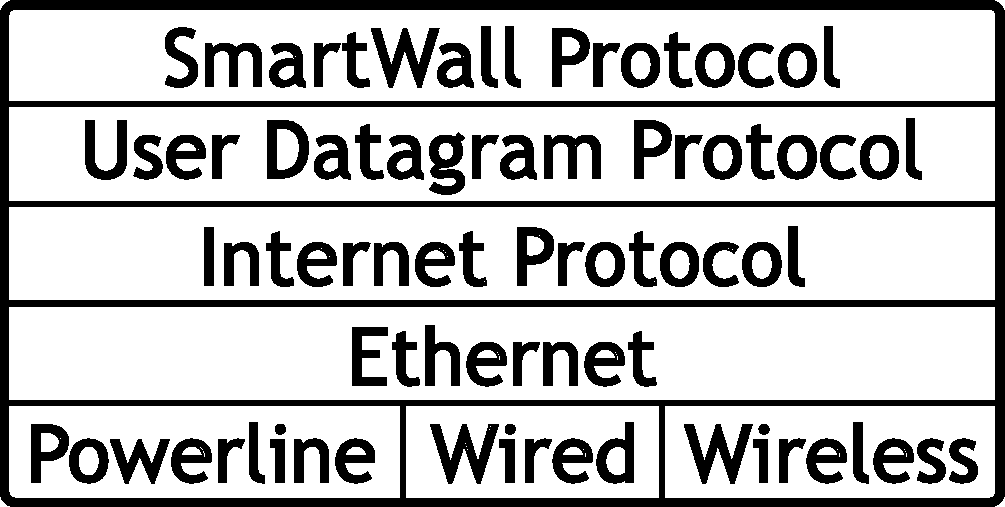
\includegraphics[scale=.5]{stack.pdf}
  \end{center}
  \caption{SmartWall Protocol Stack}
  \label{fig:swStack}
\end{figure}

\subsubsection{Mode of Operation}
\label{sec:Design.SmartWallProtocol.ModeofOperation}
The SmartWall protocol is designed to operate in a loose master/slave
configuration where all normal messages are acknowledged with the
appropriate response. Figure \ref{fig:swMode} shows this operation.

Normally, most SmartWall devices are operating in a
Slave mode. In this mode, the device passively listens for messages
addressed to it. When it receives a message, it performs the necessary
actions and sends the necessary response. Slave devices do not initiate
any message exchanges (except during self-configuration, see Section
\ref{sec:Design.SmartWallProtocol.SelfConfiguration}).

Each SmartWall network has a single active Master device at all
times. The master device on the network is in charge if initiating network
communications, normally at the request of the user interface or other
external input. The master also maintains a list of all active devices
on the SmartWall network and handles incoming configuration requests
from Slave devices (see Section
\ref{sec:Design.SmartWallProtocol.SelfConfiguration}). Master devices
are capable of automatic fail-over operation. Although there can only
be one acting Master on each SmartWall network, multiple backup masters
may be present and begin operation if the acting master fails. This
provides the ability to build highly redundant SmartWall networks for
high reliability critical applications.

\begin{figure}
  \begin{center}
    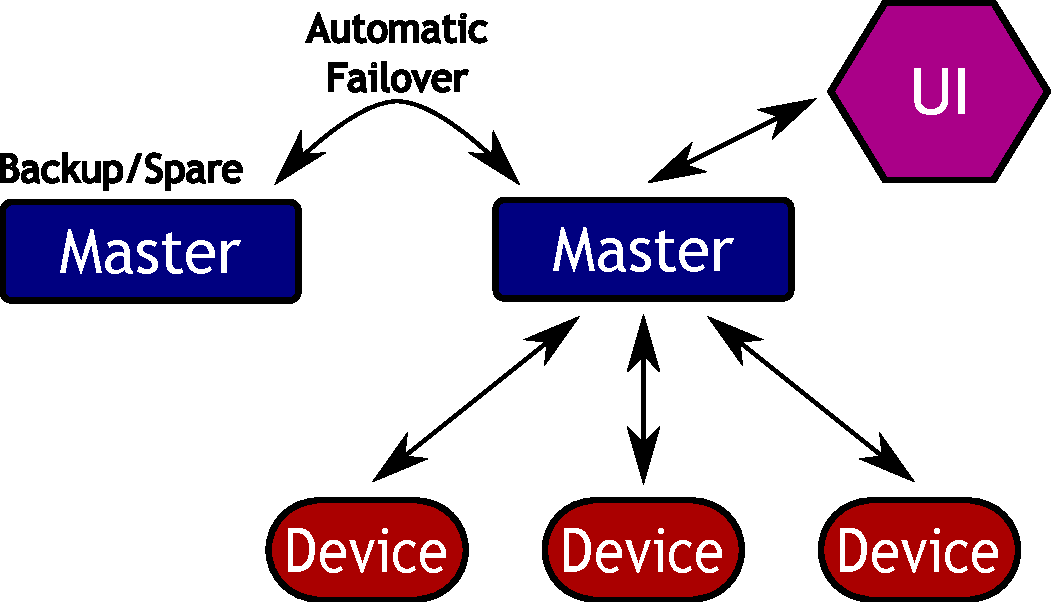
\includegraphics[scale=.5]{networkmode.pdf}
  \end{center}
  \caption{SmartWall Protocol Mode of Operation}
  \label{fig:swMode}
\end{figure}

\subsubsection{Self Configuration}
\label{sec:Design.SmartWallProtocol.SelfConfiguration}
In order to ensure ease of use, the SmartWall network is
self-configuring. To achieve this functionality, the acting Master device
on each SmartWall network is in charge providing slave devices with
the necessary
initialization and configuration parameters. When a new device is
added to the SmartWall network, it broadcasts a request for
initialization. The acting Master answers this request by sending the
appropriate configuration information. Only one device on the network
may complete the initializing process at a time. If a second device
tries to initialize while a current initialization is underway, both
initializations fail and the devices retry the initialization
procedure at random
intervals until one secures the initialization lock and successfully
completes the procedure, allowing the second device to proceed.

\subsection{SmartOutlet}
\subsubsection{Connectivity}
SmartOutlets will connect to the SmartWall network via
Ethernet-over-power-line technology, avoiding the need for extra
in-wall wiring.  Because the SmartOutlet is a
real-time-operating-system, the embedded code of the MCU must be
robust and efficient to ensure that all queries are executed in a
timely fashion, and that no data is lost.

\subsubsection{Physical Design}
In an effort to make the SmartOutlet easy to install and operate, all
of the circuitry of the device should fit inside the same
housing of a normal outlet. Once installed, the outlet will appear
identical to a normal wall outlet with the exception of a status LED
and reset button for troubleshooting and user configuration.

Future plans for the
SmartOutlet include a version with a sleek housing that does not
replace a regular electrical outlet, but instead plugs into one and
remains flat and flush against the wall.  This would make installation
even easier, and would allow the user to easily move SmartOutlets
around to different nodes in the house is situations where in-wall
retrofitting are undesirable.

\subsubsection(Electrical Design)
The SmartOutlet must also be as robust as a standard wall-outlet. This
means that the additional circuity necessary for power monitoring and
switching must be capable of operating for the 10+ year lifespan of
a standard outlet. To achieve this, we will be using solid-state
relays for switching, and where available, robust IC solutions for power
monitoring and SmartWall communication. All SmartOutlet circuitry will be
power by an integrated AC-to-DC converter that pulls power directly
from the AC power lines connected to the device. The device will
utilize energy efficient ICs and programmatic power saving modes to avoid
unnecessary energy leaching by the device itself.

Figure \ref{fig:outletDiagram} shows the system level connections and
interactions of the SmartOutlet components.

\begin{figure}
  \begin{center}
    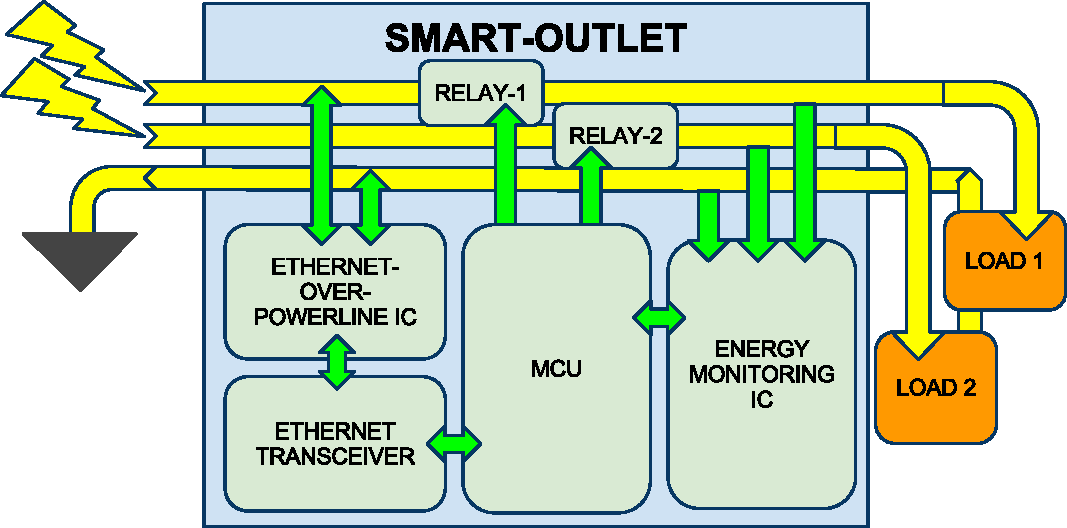
\includegraphics[scale=.5]{outletdiagram.pdf}
  \end{center}
  \caption{SmartOutlet System Diagram}
  \label{fig:outletDiagram}
\end{figure}

\subsection{User Interface}
\subsubsection{Web Based UI}
In the case of our SmartWall project, the user interface will be a
web application. For our product to be successful, the users
should find interaction with the website so intuitive that no
training or direction is needed. A web user interface has a number of
advantages over a dedicated user interface program. These include:
\begin{itemize}
  \setlength{\itemsep}{0pt}
  \setlength{\parskip}{0pt}
  \setlength{\parsep}{0pt}
\item The ability to access the UI through any device that provides a
  standardized web browser (computer, phone, etc).
\item The ability to publicly serve the interface, making it
  remotely accessible from the Internet.
\end{itemize}  

\subsubsection{Functionality}
The user interface will interact with the SmartWall Master device. It
provides the user with the necessary tools to utilize the SmartWall
network to monitor and control devices. In addition to the basic
SmartWall functionality, the user interface implements additional
functionality including:
\begin{itemize}
  \setlength{\itemsep}{0pt}
  \setlength{\parskip}{0pt}
  \setlength{\parsep}{0pt}
\item The ability to log, graph, and view energy use and device state
  over time.
\item The ability to automate device control via timers and event
  sequences.
\item The ability to alias devices with human-readable names and
  locations, and notes.
\end{itemize}  

\section{Implementation}
\subsection{Protocol}
\subsubsection{Definition and Interfaces}

The bulk of the SmartWall protocol is defined in the SmartWall
definition document in Appendix A (Section \ref{sec:AppendixA}). The
SmartWall protocol is implemented in ANSI C. Appendix B (Section
\ref{sec:AppendixB}) contains the C header files describing the protocol
and its interface.

SmartWall.h (Listing
\ref{lst:SmartWall.h} in Section \ref{sec:AppendixB.SmartWall.h}) is
the primary C header file describing the protocol definition. The
protocol defines a generic SmartWall header, as well as message scope
headers.

The SmartWall protocol utilizes the Berkeley Sockets API for accessing
the UDP/IP network stack. SmartWallSockets.h (Listing
\ref{lst:SmartWallSockets.h} in Section
\ref{sec:AppendixB.SmartWallSockets.h}) is the C header file containing
the SmartWall Sockets Interface.

\subsubsection{Key Concepts}

Each SmartWall message consists of the following:
\begin{description}
  \setlength{\itemsep}{0pt}
  \setlength{\parskip}{0pt}
  \setlength{\parsep}{0pt}
\item[SmartWall Message Header:] Contains all necessary SmartWall
  addressing and message information.
\item[SmartWall Scope Header:] Contains the necessary scope-specific
  message information. Message scopes define how wide an area a
  message governs and thus also control what the format of the message
  body looks like.
\item[SmartWall Message Body:] Contains the actual message information.
\end{description}

The formats and field descriptions for the previous items can be found
in Appendix A (Section \ref{sec:AppendixA}).

Each SmartWall device implements one or more device
type profiles. These profiles define how the device interprets a
specific opcode. By making all opcodes profile based, we ensure that
the SmartWall protocol remains extensible. If support for a new device
type is needed, one must simply add a new device type profile. By
allowing devices to implement multiple type profiles, we avoid the need
for redundant opcodes and function implementation. For example, any
device that requires simple power monitoring and the ability to turn
on and off may implement the Outlet profile, regardless of whether or not
it also supports functionality above and beyond a basic outlet.

\subsection{Reference Master}
\label{sec:Implementaion.ReferenceMaster}
In addition to the basic protocol and interface implementation, our
efforts also involved writing a reference Master implementation. This
implementation is designed to run on a standard GNU/Linux
platform. The C header files for this implementation are in Appendix C
(Section \ref{sec:AppendixC}).

The external interface to Master implementation is provided through a
series of utility programs. These programs allow one to send and
receive messages and list the active devices on the SmartWall
network. They are designed to be called at the command line directly by
the user, or indirectly called from the more advanced web based user
interface. At this time, the following utilities are provided:
\begin{description}
  \setlength{\itemsep}{0pt}
  \setlength{\parskip}{0pt}
  \setlength{\parsep}{0pt}
\item[swls:] Lists all active SmartWall devices and their information.  
\item[swChnMsg:] Sends a SmartWall Channel Scope message and returns
  the response.
\end{description}

\subsection{Reference Slave}
\label{sec:Implementaion.ReferenceSlave}
We have also coded a reference slave implementation for our SmartOutlet
device. This implementation can run as either a software based
SmartOutlet simulator, or as embedded code on the actual SmartOutlet
hardware device. The C header files related to the slave implementation
can be found in Appendix D (Section \ref{sec:AppendixD}).

\subsection{SmartOutlet}

Figure \ref{fig:outletFront} shows a concept view of the SmartOutlet device.

\begin{figure}
  \begin{center}
    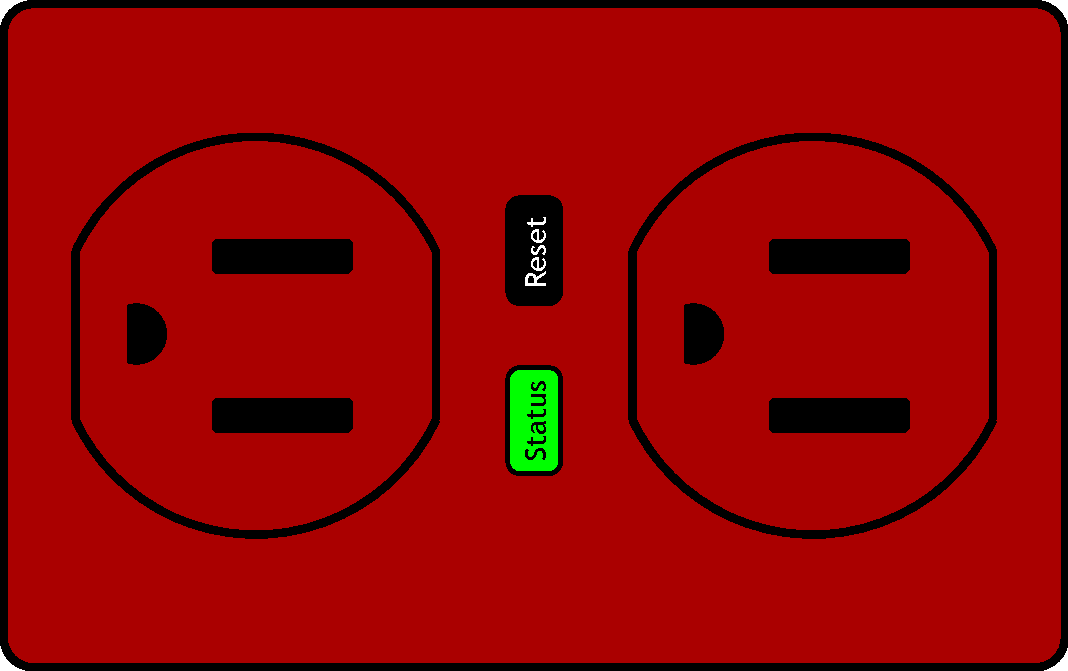
\includegraphics[scale=.5]{outlet.pdf}
  \end{center}
  \caption{SmartOutlet Front View}
  \label{fig:outletFront}
\end{figure}

The SmartOutlet prototype uses PIC32 Ethernet Starter Kit to control
all of its communications and operations. This kit provides a PIC32
MCU and the necessary Ethernet connections. The initial prototype
utilizes standard wired Ethernet, as opposed to power-line Ethernet
technology that later prototypes and the final product intent to use.

The SmartOutlet measures power by using the MCP3909 IC and some
external circuitry.  The voltage is measured using a voltage divider
across in parallel with each load, and the current is measured by
measuring the voltage produced across a
very accurate resistor in series with each load.
The MCP3909 produces digital voltage and current
readings that are sent to the PIC32 MCU via the Serial Peripheral
Interface (SPI). The MCU uses the digital samples of voltage and
current to calculate the active power being used by the loads.

Solid-state relays that capable of handling large
voltages and currents and operating with a control
voltage of 2-5V are used to switch each port of the SmartOutlet.
The states of the two ports are held in two
global variables in the embedded code (1 for on, 0 for off).  The
variables are changed based off SET messages from the SmartWall
network or reported via QUERY messages from the SmartWall network.

The overall design of the embedded code is relatively simple.
It consists of some initial setup code and a cooperative multitasking
body  loop that runs a number of state machines.
The setup phase consists of
initializing the IP stack and the SPI, and configuring the MCP3909 to
send the digital readings of its ADC converters to the MCU via the
SPI. The body state machines handle all IP communication tasks, all IP
core tasks, update the state of the outlet ports, and measures the
power being used by the loads. The SmartWall portions of the
SmartOutlet run the same code as the Reference Slave (Section
\ref{sec:Implementaion.ReferenceSlave}).

\subsection{User Interface}
\subsubsection{Parts}
The web user interface was implemented using the following software:
\begin{description}
  \setlength{\itemsep}{0pt}
  \setlength{\parskip}{0pt}
  \setlength{\parsep}{0pt}
\item[Apache2:] Web server to host the website
\item[Perl:] Scripting language which queried for and stored power usage
  data for each outlet
\item[PHP5:] Web programming language used to interface with the network
  protocol and generate some of the dynamic content of the website
\item[HTML:] Web programming language into which PHP code was embedded
\item[CSS:] Style sheet language used to make the website visually appealing
\end{description}

\subsubsection{Web Pages}
The web pages of the SmartWall prototype user interface are
implemented in php and html. They communicate with the utility
programs described in Section \ref{sec:Implementaion.ReferenceMaster}
to obtain lists of all devices on
the system and query for their on/off status and power usage.
\begin{description}
  \setlength{\itemsep}{0pt}
  \setlength{\parskip}{0pt}
  \setlength{\parsep}{0pt}
\item[Home Page:] Allows the user to view all their devices, turn them on and
off, and view the system’s total power usage.
\item[Energy Usage:] Provides user with ability to view the power usage
of each device and each channel of each device individually.
\item[Setup Page:] Allows user to identify the location of devices in their
home and rename them for convenience.
\item[Timers Page:] Would allow the user to set timers for each device.
\end{description}

\subsubsection{Power Monitoring}
Perl scripts collect power usage data and turn them into user-friendly
graphs to be displayed on the website. Every minute the scripts query
the Master for a list of devices and query each device for their
instantaneous power usage. Every five minutes, the information
collected is turned into graphs. In this manner, recent graphs are
ready and waiting when the user opens the website.

\section{Results and Examples}
\subsection{Reference Protocol and Device Implementation}

The example output of the swls Master utility can be found in Listing
\ref{lst:swls.txt}. This output shows the list of SmartWall devices on
the local host, the types and address of each device, and various
other device specific information necessary to communicate with each device.

\lstinputlisting[language=bash,
  caption={swls Example Output},
  label=lst:swls.txt]{swls.txt}

Listing \ref{lst:swChnMsg.txt} shows the example output of an exchange
of SmartWall message between the Master device and a local slave
outlet device via the swChnMsg command. We first query the slave
outlet for the on/off state of each of its two sockets. We then set
each socket to the ``On'' state. Finally, we query the outlet a second
time to confirm that each socket is indeed ``On''. The outlet replies
to each message from the master with a report of the current state of
the affected channels.

\lstinputlisting[language=bash,
  caption={swChnMsg Exchange Example Output},
  label=lst:swChnMsg.txt]{swChnMsg.txt}

Listing \ref{lst:msg1-2.txt} is a dump of the network packet traffic
involved in the first Query/Response exchange shown in Listing
\ref{lst:swChnMsg.txt}. For a full packet dump of the entire
Listing \ref{lst:swChnMsg.txt} message exchange, see Appendix E (Section
\ref{sec:AppendixE}).

\lstinputlisting[language=bash,
  caption={swChnMsg Exchange Network Packets 1 and 2},
  label=lst:msg1-2.txt]{msg1-2.txt}

\subsection{SmartOutlet}
The current prototype of the SmartOutlet is able to communicate with
the SmartWall network and control the states of the electrical ports of the
outlet. Power monitoring functionality has not been entirely
implemented due to complications with the SPI.

The current prototype
outlet is not wired to measure power produced by normal residential AC
voltage and current levels, though the relays used to
control the state of the outlet ports are capable of handling such
levels.  The circuitry for the prototype SmartOutlet is powered by a
connected USB cable or AC adapter and is capable of switching 24V DC
loads.

\subsection{Web Interface}

The final result for the user interface was a php and html website
which allowed the user to view all devices connected to their system,
along with their on/off status, turn each channel of each device on
and off at will, and view the power usage of the system as a whole
and of each outlet individually. Some infrastructure was also put in
place for setting timers and aliasing/renaming outlets for ease of
use. Aliases could be displayed if hard-coded, but the ability to
rename outlets through the website was not completed.

Shown in Figure \ref{fig:webUI-home} is the website homepage. It provides the
user with immediate access to a list of all the devices in their
home, whether each device is on or off, the ability to turn each
device on or off, and a graph of the system's power usage for the
past month. 

\begin{figure}
  \begin{center}
    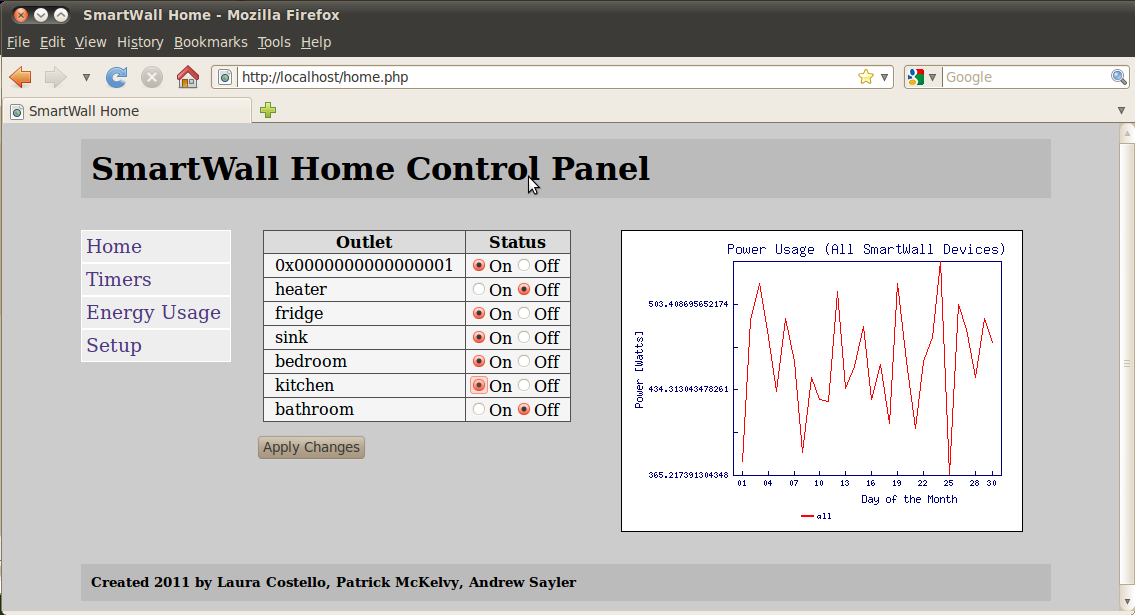
\includegraphics[scale=.3]{webUI-home.png}
  \end{center}
  \caption{UI - Device Control Home Page}
  \label{fig:webUI-home}
\end{figure}

Shown in Figure \ref{fig:webUI-energy} is the page that allows users
to view power usage on
a per-device basis. The user can select the device they wish to
view information about and see a graph of the past month’s power
usage. The two lines on the graph show the two sockets or
channels of an outlet, which are independently controllable. 

\begin{figure}
  \begin{center}
    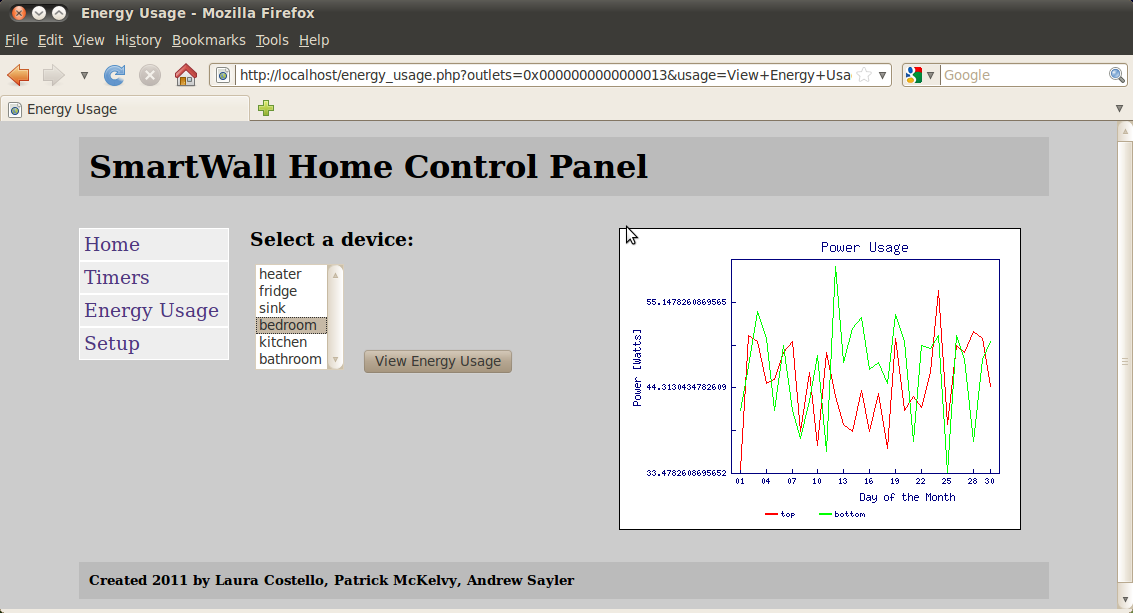
\includegraphics[scale=.3]{webUI-energy.png}
  \end{center}
  \caption{UI - Monitor Device Energy Usage History}
  \label{fig:webUI-energy}
\end{figure}

Interacting with the
Engineering Psychology consultants assigned to our group was also an
important part of the interface design. We met with
them as a whole group shortly after they were assigned to us in order
to bring them up to speed on our project. We explained our premise
and goals for the project and set out a tentative schedule for
further communications. As we designed the website, we interacted
with them several times order to get feedback. After giving them
goals for the user interface, we solicited suggestions on what a user
might want to see first when they open the website. They suggested
that the list of device and a graph of the overall energy usage would
be most valuable, and we implemented the homepage with these
suggestions in mind. As the website began to take shape, we met with
them twice more to demonstrate and solicit suggestions on what could
be changed or improved to make it more user-friendly. Their
suggestions regarding layout and vocabulary were incorporated into
the final design. 

\section{Analysis}



\section{Conclusion}


\section{Recommendations}


\renewcommand{\refname}{\section{References}}
\begin{thebibliography}{10}

\bibitem{RFC1958} Internet Engineering Task Force: Network Working Group.
  \newblock ``RFC 1958''.
  \newblock Brian Carpenter, Editor.
  \newblock (June 1996).
  \newblock \url{http://datatracker.ietf.org/doc/rfc1958/}.

\bibitem{CNID} Metcalfe, RM.
  \newblock ``Computer Network Interface Design: Lessons from
  Arpanet and Ethernet''.
  \newblock IEEE Journal on Selected Areas in Communications.
  \newblock (February 1993).

\bibitem{artUnix} Raymond, Eric S.
  \newblock \emph{The Art of Unix Programming}.
  \newblock Boston: Addison-Wesley, 2004.

\bibitem{p3-KillAWatt} P3 International.
  \newblock ``P4400 Kill A Watt''.
  \newblock Retrieved 2004 EST, May 1, 2011.
  \newblock \url{http://www.p3international.com/products/special/P4400/P4400-CE.html}

\bibitem{compNetworks} Tanenbaum, Andrew S.
  \newblock \emph{Computer Networks}. 4th ed.
  \newblock Upper Saddle River, NJ: Prentice Hall PTR, 2003.

\bibitem{googleStory} Vise, David A., and Mark Malseed.
  \newblock \emph{The Google Story}.
  \newblock New York, NY:Delacorte, 2008.
  \newblock Google Books.
  \newblock \url{http://books.google.com}.

\bibitem{wiki-X10} ``X10 (industry standard)''.
  \newblock Wikipedia, The Free Encyclopedia.
  \newblock 2011, April 29.  Retrieved 1953 EST, May 1, 2011.
  \newblock \url{http://en.wikipedia.org/w/index.php?title=X10_(industry_standard)&oldid=426496014}.

\bibitem{UIDesign} Wood, Larry E.
  \newblock \emph{User Interface Design: Bridging the Gap from User
    Requirements to Design}.
  \newblock Boca Raton: CRC, 1998.
  \newblock Google Books.
  \newblock \url{http://books.google.com>}.

\end{thebibliography}

\pagebreak

\section{Appendix A - Protocol Definition}
\label{sec:AppendixA}

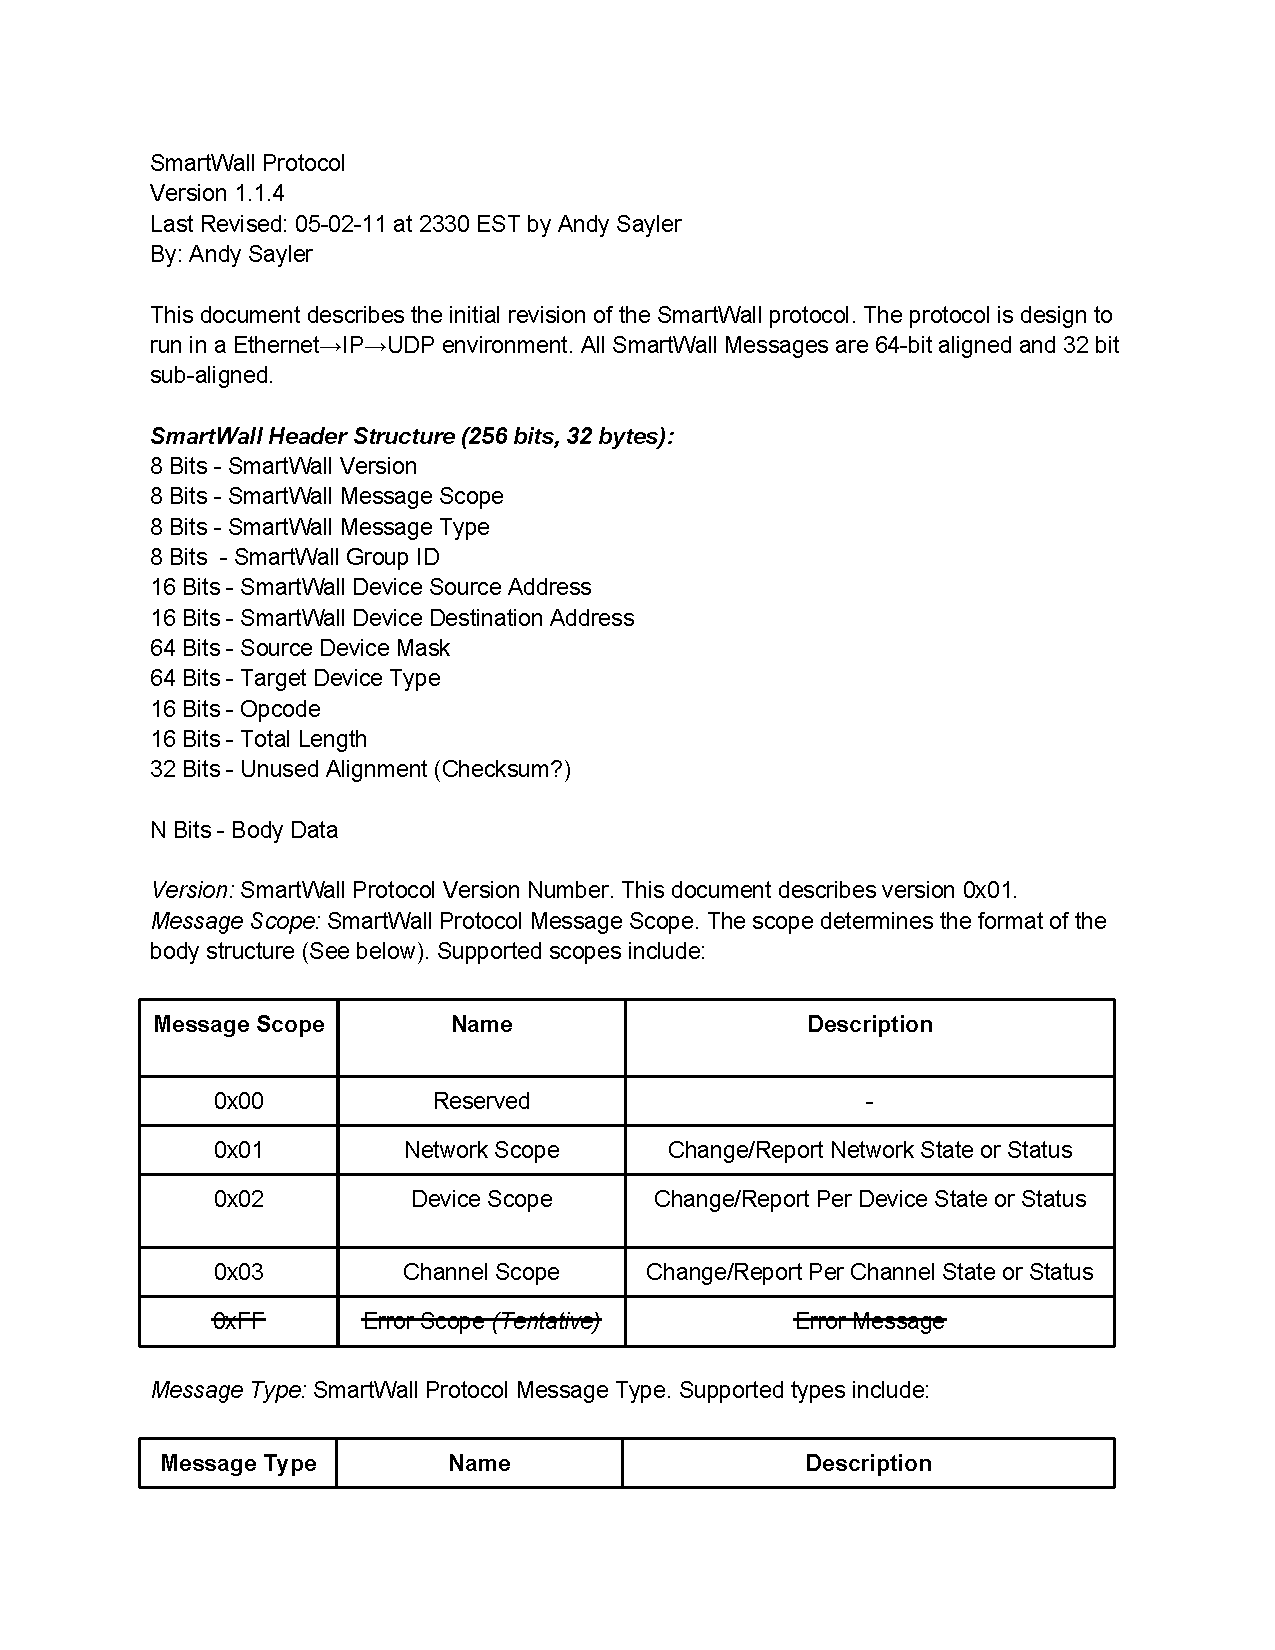
\includepdf[pages={1-4}]{SmartWallVersion1.pdf}

\pagebreak

\section{Appendix B - Protocol and Common Headers}
\label{sec:AppendixB}

\pagebreak

\subsection{SmartWall.h}
\label{sec:AppendixB.SmartWall.h}
\lstinputlisting[language=C,
  caption={SmartWall Protocol Definition - SmartWall.h},
  label=lst:SmartWall.h]{../com/SmartWall.h}

\pagebreak

\subsection{SmartWallSockets.h}
\label{sec:AppendixB.SmartWallSockets.h}
\lstinputlisting[language=C,
  caption={SmartWall Sockets Interface - SmartWallSockets.h},
  label=lst:SmartWallSockets.h]{../com/SmartWallSockets.h}

\pagebreak

\subsection{comTools.h}
\label{sec:AppendixB.comTools.h}
\lstinputlisting[language=C,
  caption={SmartWall Auxiliary Tools - comTools.h},
  label=lst:comTools.h]{../com/comTools.h}

\pagebreak

\subsection{comPrint.h}
\label{sec:AppendixB.comPrint.h}
\lstinputlisting[language=C,
  caption={SmartWall Print Functions - comPrint.h},
  label=lst:comPrint.h]{../com/comPrint.h}

\pagebreak

\subsection{swDevice.h}
\label{sec:AppendixB.swDevice.h}
\lstinputlisting[language=C,
  caption={SmartWall Device Interface - swDevice.h},
  label=lst:swDevice.h]{../com/swDevice.h}

\pagebreak

\section{Appendix C - Master Implementation}
\label{sec:AppendixC}

\pagebreak

\subsection{swMaster.h}
\label{sec:AppendixC.swMaster.h}
\lstinputlisting[language=C,
  caption={SmartWall Master Interface Header - swMaster.h},
  label=lst:swMaster.h]{../master/swMaster.h}

\pagebreak

\section{Appendix D - Slave Implementation}
\label{sec:AppendixD}

\pagebreak

\subsection{swSlave.h}
\label{sec:AppendixD.swSlave.h}
\lstinputlisting[language=C,
  caption={SmartWall Slave Interface Header - swSlave.h},
  label=lst:swSlave.h]{../slave/swSlave.h}

\pagebreak

\subsection{swUniversal.h}
\label{sec:AppendixD.swUniversal.h}
\lstinputlisting[language=C,
  caption={SmartWall Universal Device Interface Header - swUniversal.h},
  label=lst:swUniversal.h]{../slave/swUniversal.h}

\pagebreak

\subsection{swOutlet.h}
\label{sec:AppendixD.swOutlet.h}
\lstinputlisting[language=C,
  caption={SmartWall Outlet Device Interface Header - swOutlet.h},
  label=lst:swOutlet.h]{../slave/swOutlet.h}

\pagebreak

\section{Appendix E - Example SmartWall Message Exchange}
\label{sec:AppendixE}

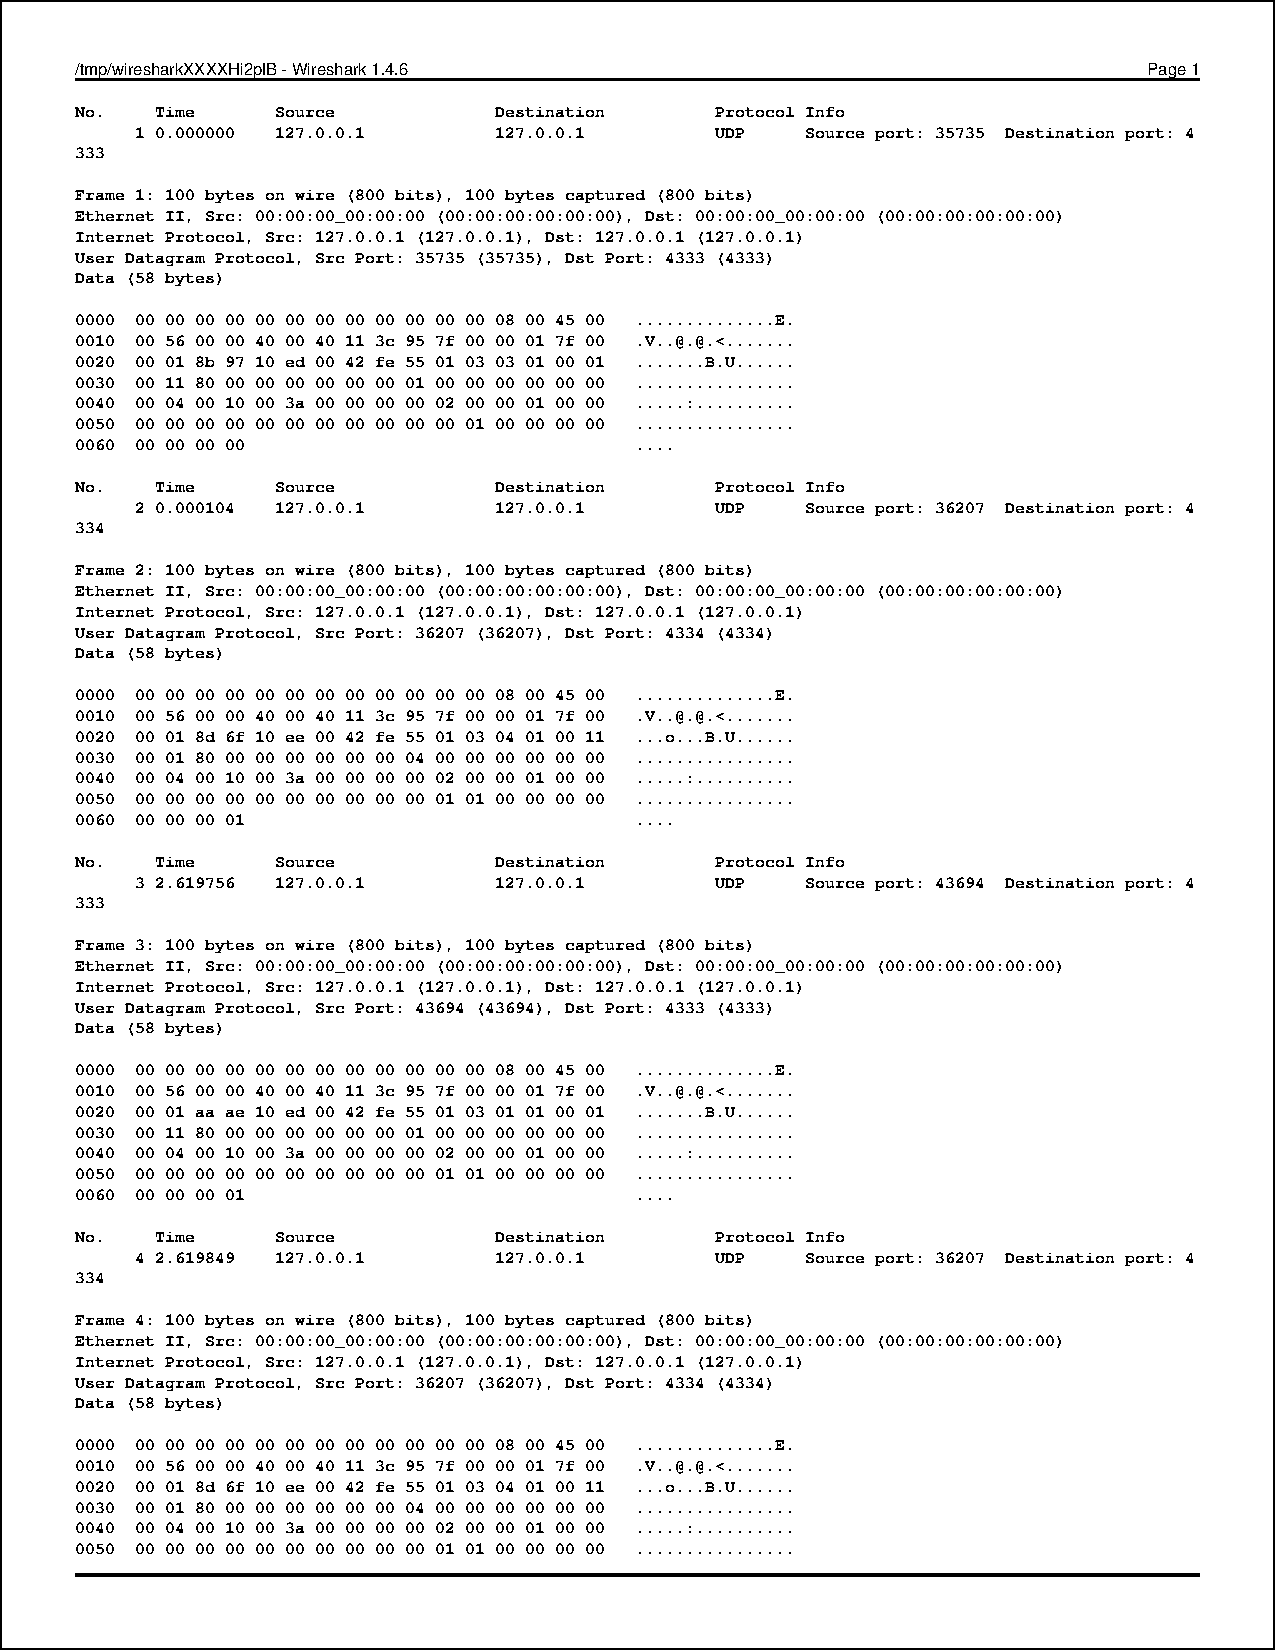
\includepdf[pages={1-2}]{msgExchange.pdf}

\pagebreak


\end{document}
